%  !TeX  root  =  user_guide.tex

\section{ Plugin SQL Anywhere}\label{sec:sqlanywhere}

% when the revision of a section has been finalized, 
% comment out the following line:
% \updatedisclaimer

SQL Anywhere è un database relazionale proprietario (RDBMS) prodotto da Sybase. 
Fornisce supporto ai dati geospaziali, es. OGC e shapefile, e consente di esportare 
nei formati KML, GML e SVG.

Il fornitore dati SQL Anywhere \toolbtntwo{sqlanywhere}{Aggiungi un layer SQL anywhere} 
presente in QGIS è rilasciato con licenza GPL v3. 
La finestra di dialogo \dialog{Aggiungi un layer SQL anywhere} è simile nelle funzionalità a quella di PostGIS 
e a quella di SpatiaLite.

\begin{figure}[ht]
   \centering
   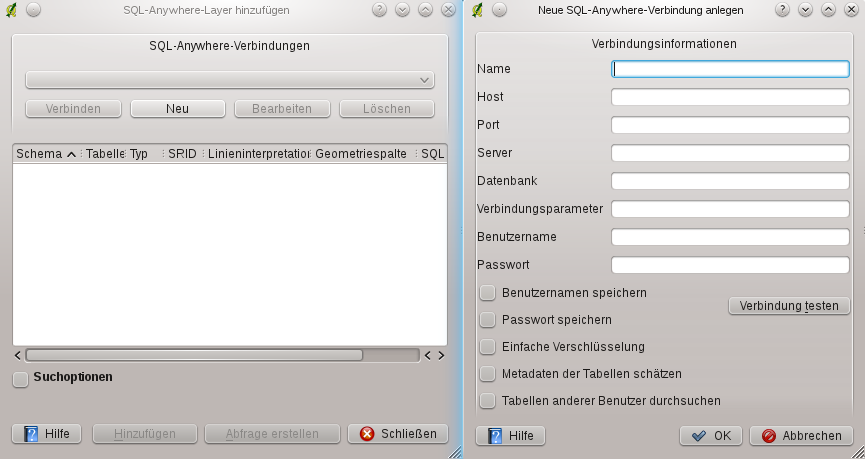
\includegraphics[clip=true, width=14cm]{sql_anywhere}
   \caption{Finestra di dialogo SQL Anywhere \wincaption}
   \label{fig:sqlanywhere}
\end{figure}

%% FIXME Needs an example, but the database is proprietary

\FloatBarrier
